\documentclass[a4paper, 12pt]{article}
\usepackage{csquotes}
\usepackage{titlesec}
\usepackage[ngerman]{babel}
\usepackage[a4paper, left=3cm, right=3cm, top=2cm, bottom=2cm]{geometry}
\usepackage{fouriernc}
\usepackage{titlesec}
\usepackage{keystroke}

\newcommand{\makeTitleAndTable}{
    \begin{titlepage}
        \centering
        \vspace*{1.5cm}
        {\Huge Einfacher SPH Flüssigkeitssimulator mit Beschleunigter Nachbarschaftssuche\par}
        \vspace{1cm}
        {\LARGE Thierry Meiers\par}
        {\Large Bachelor Projekt\par}
        \begin{figure}[H]
            \centering
            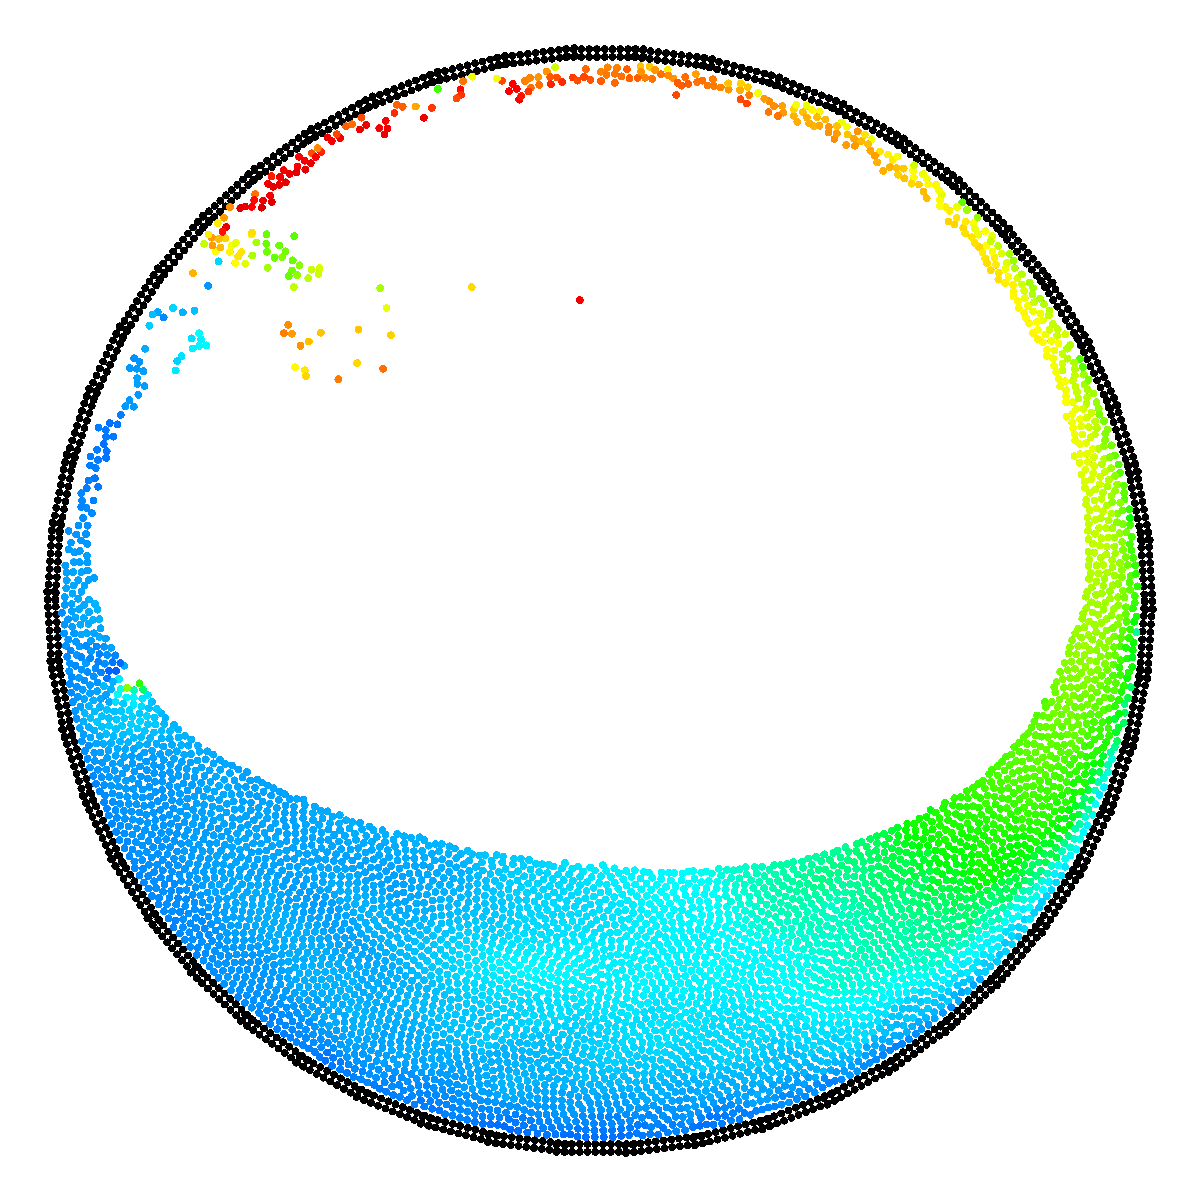
\includegraphics[width=.7\textwidth]{graphics/FirstPage.png}
        \end{figure}
        \vspace{0.5cm}
        {\large Albert-Ludwigs-Universität Freiburg\\Technische Fakultät\\Graphische Datenverarbeitung\par}
        \vfill
        {\large \today \par}
    \end{titlepage}
    \pagenumbering{gobble}
    \tableofcontents
    \clearpage
    \pagenumbering{arabic}
}

\usepackage[ngerman]{babel}
\usepackage[dvipsnames]{xcolor}
\usepackage{graphicx} 
\usepackage{microtype}
\usepackage{subcaption}
\usepackage{float}
\usepackage{parskip}
\usepackage{amsmath}
\usepackage{hyperref}
\usepackage{enumitem}
\begin{document}

\makeTitleAndTable

\section{Einführung}
Fluidsimulationen haben sich zu einem unverzichtbaren Werkzeug in zahlreichen Bereichen unserer Gesellschaft entwickelt. Sie ermöglichen die präzise Simulation von Flüssigkeiten oder Gasen in verschiedenen Umgebungen, wodurch das Verhalten dieser Stoffe und deren Interaktionen mit der Umgebung untersucht werden können. Aufgrund ihrer Vielseitigkeit kommen Fluidsimulationen in einer großen Bandbreite von Anwendungsgebieten zum Einsatz. Diese reichen von der Optimierung von Fahrzeugen und Gebäuden über Wettervorhersagen und medizinische Forschung bis hin zur Erzeugung realistischer Effekte in Filmen und Spielen, industriellen Prozessen, Energieerzeugung und der Entwicklung von Sportgeräten. Sie tragen wesentlich dazu bei, Designs zu verbessern, die Effizienz zu steigern und komplexe Strömungen besser zu verstehen. Die Allgegenwärtigkeit und Bedeutung dieser Technologie in verschiedenen Branchen haben mein Interesse an diesem Thema geweckt. Insbesondere die Verbindung von Physik und Informatik ist eine Motivation zur Arbeit an diesem Projekt.
Das Hauptziel dieses Projektes ist die Implementierung und Analyse der Smoothed Particle Hydrodynamics (SPH) zur Simulation von Fluiden und dabei ein tieferes Verständnis für die Komponenten und Mechanismen von SPH zu entwickeln.

\section{Navier-Stokes equations}

\section{Smoothed Particle Hydrodynamics}

\section{Implementierung}
\subsection{Simulation}
\subsection{Nachbarschaft Suchen}
\subsection{Oberflächenspannung}

\section{Analysen}

\section{Schlussfolgerung}

\section{Bibliographie}
\end{document}